% =====================================================================
% 2. Data pipeline (T5, MM: summary) and EDA implementation (T6, own)
% =====================================================================
\section{Data pipeline and exploratory analysis}\label{sec:data-code}

\subsection{Data pipeline (Mar\'ia's block, summary)}

The data block (task T5, done by Mar\'ia and reviewed by me) turns the PhysioNet files into PyTorch
batches:
\begin{enumerate}[leftmargin=1.4em,itemsep=1pt]
  \item \textbf{Integrity.} Every file used is hashed with SHA-256 and compared with the checksum list
        published with the dataset, so the cache is built only from unaltered files.
  \item \textbf{Labels.} A multi-hot float matrix (records $\times$ 5) in the order NORM, MI, STTC, CD,
        HYP, with the rule of the script distributed with PTB-XL; a test compares the class counts with
        the table of the PhysioNet page.
  \item \textbf{Cache.} Each record is read once with \texttt{wfdb}, checked (100\,Hz, the 12 expected
        leads, 1000 samples) and stored as $(12, 1000)$, the (channels, time) layout that
        \texttt{Conv1d} expects, together with labels, identifiers, fold and a flag for records without a
        superclass, in one compressed NumPy file. It is written to a temporary file and renamed, so an
        interrupted run never leaves half a cache.
  \item \textbf{Splits and normalisation.} Folds 1--8 / 9 / 10; per-lead mean and standard deviation
        over the training records only, applied to the three splits. Computing them on validation or test
        records would leak information about them.
  \item \textbf{Dataset and DataLoader.} \texttt{\_\_len\_\_} and \texttt{\_\_getitem\_\_} return one
        $(x, y)$ pair; the Dataset keeps a reference to the full array and a list of row indices, so the
        splits do not copy the data; only the training loader shuffles, with a seeded
        \texttt{torch.Generator}. \texttt{num\_workers=0}, because on Windows each worker process would
        copy the in-memory cache. A batch has shape $(B, 12, 1000)$ and labels $(B, 5)$ as floats, which
        \texttt{BCEWithLogitsLoss} requires.
\end{enumerate}

\subsection{Exploratory analysis (own block)}

The EDA is one script (\texttt{src/eda.py}) and a short notebook that calls it and shows the figures.
Implementation choices worth explaining:
\begin{itemize}[leftmargin=1.2em,itemsep=1pt]
  \item \textbf{One output file.} \texttt{results/logs/eda.json} has three parts: \texttt{scalars}
        (flat name $\to$ number, read by the number generator), \texttt{tables} (small tables behind the
        figures) and \texttt{meta} (date, commit, package versions). The script rewrites everything in
        each run, so numbers and figures always come from one complete run.
  \item \textbf{Same functions as the models.} Labels and per-lead statistics are computed with the
        functions of the data loaders, and the script stops if its labels differ from the cache; the
        means and standard deviations it reports are exactly the values used for normalisation.
  \item \textbf{Co-occurrence with one product.} With the label matrix $Y$ (records $\times$ 5), $Y^\top Y$
        counts in cell $(i,j)$ the records with both classes; dividing each row by its diagonal gives
        $P(j \mid i)$, which is not symmetric (Figure~\ref{fig:eda_label_cooccurrence}).
  \item \textbf{Lazy reading.} Asking the \texttt{.npz} file for two keys loads only those arrays, not the
        signals, so the metadata analyses run in seconds.
  \item \textbf{Codings.} Age 300 means ``older than 89'' in the dataset's change log, so these records
        form a separate group left out of the medians; sex 0 is male and 1 female
        \cite[p.~6]{wagner2020ptbxl}.
  \item \textbf{Figures.} Each split, class and sex keeps one colour in every figure, the palette was
        checked for colour-blind readers, and lines also carry markers and direct labels. Example traces
        are drawn at random with a seed among single-class training records, not hand-picked.
\end{itemize}

% Shared float (common/make_floats.py). Figure: figures/eda_label_cooccurrence.pdf
\begin{figure}[htbp]
\centering
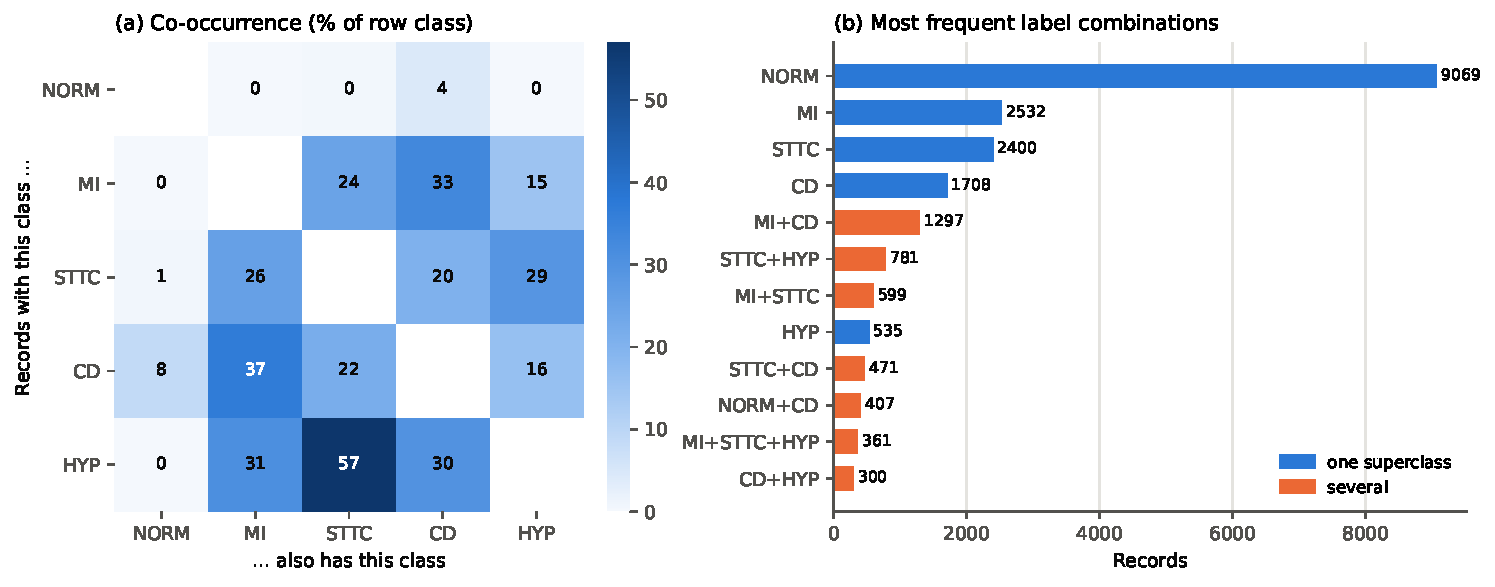
\includegraphics[width=\textwidth,height=0.42\textheight,keepaspectratio]{figures/eda_label_cooccurrence.pdf}
\caption[Co-occurrence and combinations of superclasses]{Multi-label structure. (a) Co-occurrence: percentage of the records of the row class that also carry the column class (not symmetric). (b) Most frequent label combinations; blue: one superclass, orange: several.}
\label{fig:eda_label_cooccurrence}
\end{figure}


The analysis found \edaNNanValuesTrain{} missing values and \edaNFlatLeadsTrain{} constant lead in the
training set (a lead whose metadata already notes an electrode problem); nothing was excluded. Its
conclusions for the design (records without a superclass left out, macro AUROC, sigmoid outputs,
patient-wise bootstrap, per-lead z-score) are discussed in the PRDL-DL report.
